\begin{exmp}[Lane change]
	We focus on the lane change sub-scenario of the Passing scenario, and model the ego vehicle as an HCHA.
	The closed-loop ego vehicle can be represented by the CHA of Fig.\ref{fig:LaneChangeHCHA}.
	\begin{figure}[t]
\centering
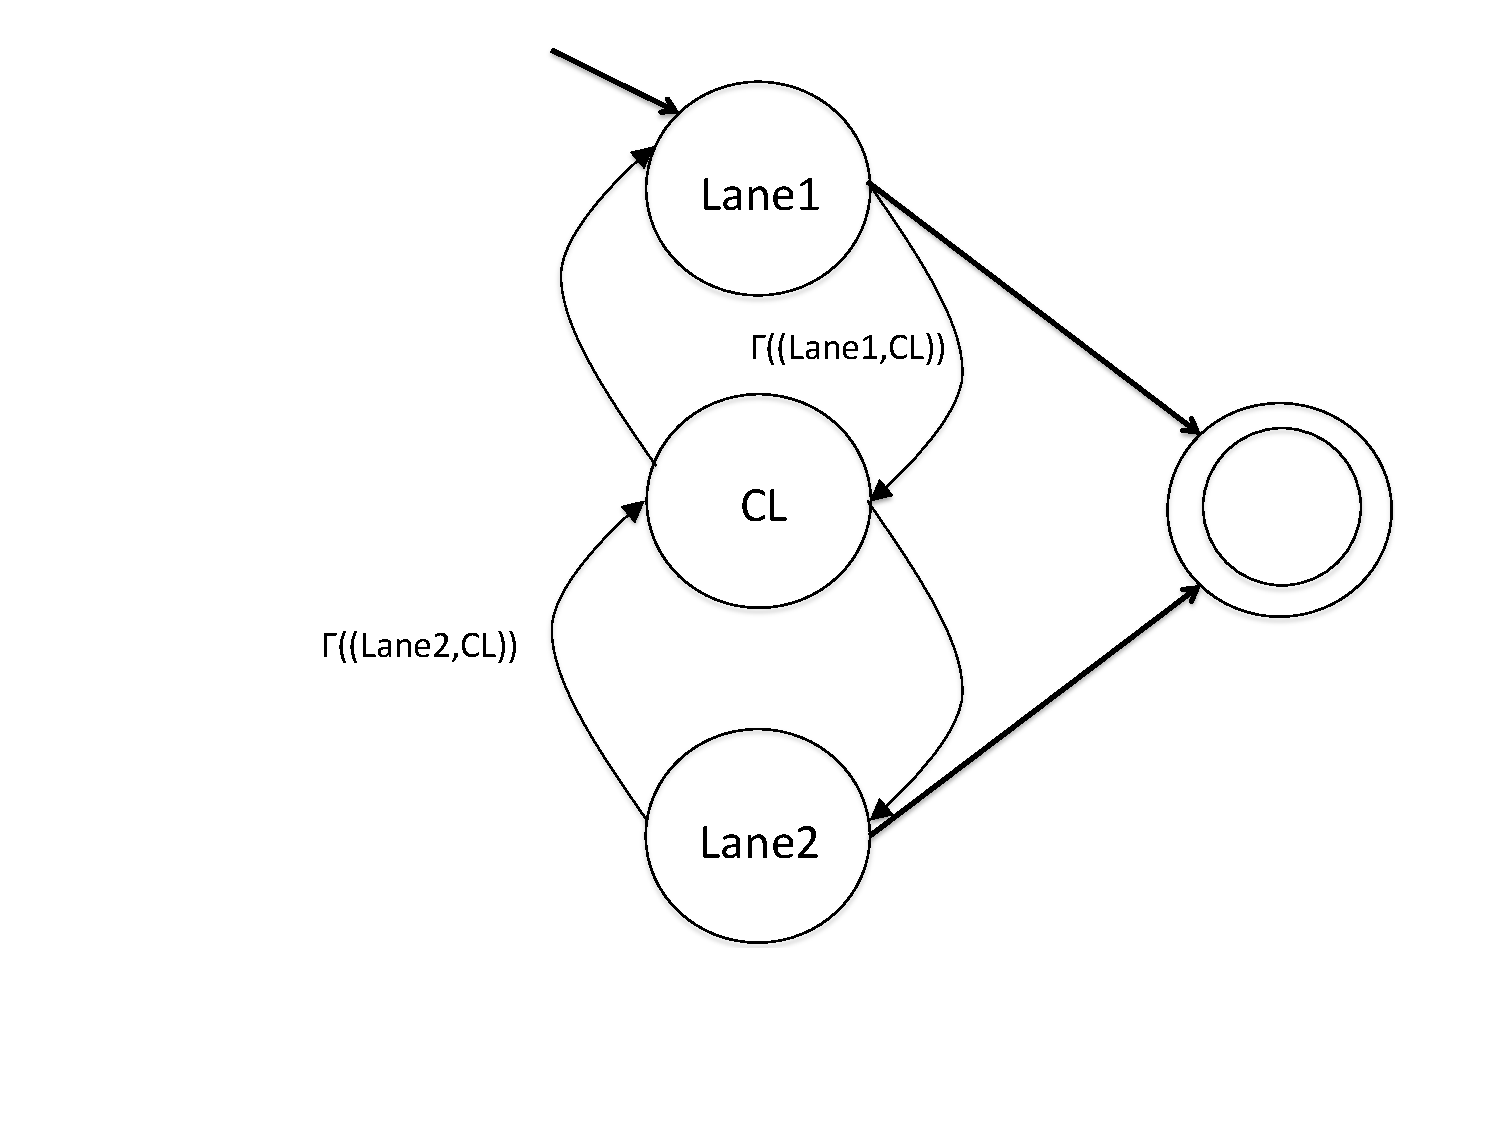
\includegraphics[scale=0.3]{figures/LaneChangeHCHA}
\caption{CHA for Ego vehicle}
\label{fig:LaneChangeHCHA}
\end{figure}
	Location $\mode_1$ indicates the vehicle is in lane 1, and $\mode_2$ indicates it is in lane 2.
	Location $CL$ is the Change Lane location.
	The state vector $x = (\beta,\Psi,\dot{\Psi}, v, s_x, s_y, \delta)$
	consists of various dynamical quantities from the \emph{bicycle model} ??? cite of a car.
	In particular, $\Psi$ is the heading angle, $v$ is the speed, and $(s_x,s_y)$ is the vehicle position.
	The continuous dynamics for the ego vehicle are identical for locations $\mode_1,\mode_2,CL$, except for a discrete jump in the heading angle $\Psi$ to effect the lane change.
	For example,
	$\reset((\mode_1,CL),x) =  (\beta,\Psi+\pi/4,\dot{\Psi}, v, s_x, s_y, \delta)$.
	See ???Matthias for details.
	The transitions $(\mode_i, CL)$ are triggered by the guard condition 
	\[\guard((\mode_i,CL)) = \{\|x_e - x_o\| \leq d \land 0 < v_o < v_e\}\]
	Guard conditions on $(CL,\mode_i)$ insure that a lane change can not be aborted (more complex models will allow maneuver interruption).
	The final state (indicated by the usual double circle) indicates some pre-determined end to the scenario, and transition into it can be guarded, for example, by a clock.
	\end{exmp}
